\documentclass[tikz,border=8pt]{standalone}
% Shared look for every TikZ diagram. Load with \input{../../tools/tikz-style.tex}
\usepackage[T1]{fontenc}
\usepackage{lmodern}
\renewcommand{\sfdefault}{lmr}  % diagrams use the same serif as the text
\usetikzlibrary{arrows.meta, positioning, shapes.geometric, calc, fit, backgrounds}
\definecolor{cblue}{HTML}{4C78A8}
\definecolor{corange}{HTML}{F58518}
\definecolor{cgreen}{HTML}{54A24B}
\definecolor{cred}{HTML}{E45756}
\definecolor{cpurple}{HTML}{B279A2}
\definecolor{cgrey}{HTML}{6B6B6B}
\tikzset{
  every picture/.style={font=\sffamily, line width=1.2pt},
  box/.style={draw=#1, fill=#1!12, rounded corners=4pt, align=center, inner sep=7pt, minimum height=1.1cm},
  box/.default=cgrey,
  arrow/.style={-{Stealth[length=3mm]}, draw=cgrey, line width=1.4pt},
  title/.style={font=\sffamily\bfseries\Large},
  note/.style={font=\sffamily\small, text=cgrey, align=center},
}
\AtBeginDocument{\hyphenpenalty=10000 \exhyphenpenalty=10000}

\begin{document}
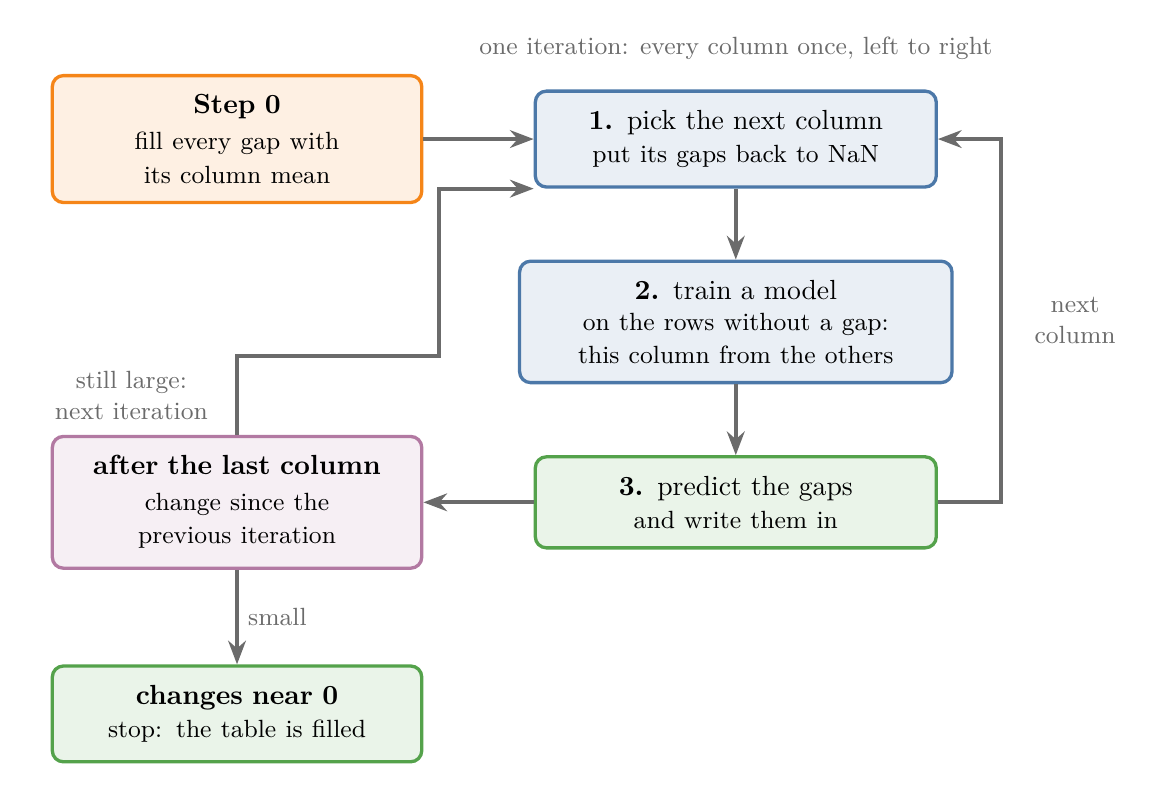
\begin{tikzpicture}[node distance=0.9cm and 1.0cm]
  \node[box=corange, text width=4.2cm] (mean) {\textbf{Step 0}\\[2pt]\small fill every gap with\\its column mean};
  \node[box=cblue, text width=4.6cm, right=1.4cm of mean] (remove) {\textbf{1.} pick the next column\\\small put its gaps back to NaN};
  \node[box=cblue, text width=5cm, below=of remove] (train) {\textbf{2.} train a model\\\small on the rows without a gap:\\this column from the others};
  \node[box=cgreen, text width=4.6cm, below=of train] (predict) {\textbf{3.} predict the gaps\\\small and write them in};
  \node[box=cpurple, text width=4.2cm, left=1.4cm of predict] (diff) {\textbf{after the last column}\\[2pt]\small change since the\\previous iteration};
  \node[box=cgreen, text width=4.2cm, below=1.2cm of diff] (stop) {\textbf{changes near 0}\\\small stop: the table is filled};
  \draw[arrow] (mean) -- (remove);
  \draw[arrow] (remove) -- (train);
  \draw[arrow] (train) -- (predict);
  \draw[arrow] (predict.east) -- ++(0.8,0) |- node[note, pos=0.25, right, text width=1.6cm] {next\\column} (remove.east);
  \draw[arrow] (predict) -- (diff);
  \draw[arrow] (diff) -- node[note, right] {small} (stop);
  \draw[arrow] (diff.north) -- node[note, left, text width=2.4cm] {still large:\\next iteration} ++(0,1.0) -| ([xshift=-1.2cm]remove.south west) -- ([xshift=0cm]remove.south west);
  \node[note, above=0.25cm of remove] {one iteration: every column once, left to right};
\end{tikzpicture}
\end{document}
